%Template Proposal PA
%Departemen Teknik Elektro dan Informatika
%Sekolah Vokasi UGM

%Dikembangkan oleh Dr. Fahmizal, S.T., M.Sc. dan Tim

%Perangkat lunak yang digunakan untuk mengolah LaTEX pada template ini adalah
%- TeXstudio
%- MiKTex
%- Overleaf (LaTEX editor berbasis daring)

\documentclass[12pt, a4paper, onecolumn, oneside, final]{report}

%Isi identitas proyek akhir disini

\providecommand{\tipe}{Proposal Proyek Akhir}
\providecommand{\permohonan}{Proposal Permohonan Proyek AKhir}
\providecommand{\judul}{(Judul Proyek Akhir yang Diajukan)}

\providecommand{\penulisPertama}{Nama Mahasiswa} 
\providecommand{\nimPertama}{XX/XXXXXX/SV/XXXXX}

\providecommand{\prodi}{Teknologi Rekayasa Elektro} 
\providecommand{\departemen}{Departemen Teknik Elektro dan Informatika}
\providecommand{\fakultas}{Sekolah Vokasi}
\providecommand{\universitas}{Universitas Gadjah Mada} 

\providecommand{\tglpengesahan}{\today} 
\providecommand{\tglpersetujuan}{\today}
\providecommand{\tglpernyataan}{\today}
\providecommand{\tahun}{\the\year{}} 

\providecommand{\tanggalSeminar}{} 
\providecommand{\waktuSeminar}{} 
\providecommand{\tempatSeminar}{} 

\providecommand{\dosenPembimbingI}{Nama Dosen Pembimbing I} 
\providecommand{\dosenPembimbingII}{Nama Dosen Pembimbing II} 
\providecommand{\ketuaProgramStudi}{Nama Ketua Program Studi} 

\providecommand{\nipDosenPembimbingI}{XXXXXXXXXXXXXXXX} 
\providecommand{\nipDosenPembimbingII}{XXXXXXXXXXXXXXXX} 
\providecommand{\nipKetuaProgramStudi}{XXXXXXXXXXXXXXXX} 

\providecommand{\katakunci}{kata kunci 1, kata kunci 2, kata kunci 3}

% Mengatur bahasa latex
\usepackage[indonesian]{babel}
\usepackage[utf8]{inputenc}

% Untuk pengaturan spacing
\usepackage{setspace}
\onehalfspacing

% Untuk mengatur level section 
\setcounter{secnumdepth}{6}

% Digunakan untuk memasukan gambar ke laporan. 
\usepackage{graphicx}
\graphicspath{{gambar/}}
\usepackage{float}
\usepackage[hang,centerlast, nooneline ,small,md]{subfigure}
\usepackage[subfigure]{tocloft}

% Untuk mengatur spacing antara paragraf
\usepackage{parskip}

% Membuat indent
\usepackage{indentfirst}
\setlength\parindent{1cm}

% Untuk mengkustomisasi margin
\usepackage{scrextend}

% Untuk mengatur header dan footer
\usepackage{fancyhdr}

% Membuat seluruh tulisan menjadi Times New Roman. 
% \usepackage{pslatex}

% Merubah numbering chapter dan section untuk judul setiap bab menggunakan romawi dan judul anak bab menggunakan arabic
\renewcommand{\thesection}{\arabic{chapter}.\arabic{section}\hspace{0.05cm}}
\renewcommand{\thesubsection}{\arabic{chapter}.\arabic{section}.\arabic{subsection}\hspace{-0.25cm}}
\renewcommand{\thesubsubsection}{\Alph{subsubsection}.\hspace{-0,25cm}}

% Mengatur identasi judul section dan subsection
%\titleformat{\section}[block]{\bfseries}{\thesection.}{1em}{}
%\titleformat{\subsection}[block]{\hspace{2em}}{\thesubsection}{1em}{}

% Merubah huruf kapital pada judul daftar isi, daftar gambar, dan daftar table
\usepackage{tocloft}
\renewcommand{\cfttoctitlefont}{\hfil\large\bfseries\MakeUppercase}
\renewcommand{\cftloftitlefont}{\hfil\large\bfseries\MakeUppercase}
\renewcommand{\cftlottitlefont}{\hfil\large\bfseries\MakeUppercase}

\renewcommand\cftchappresnum{BAB }
\renewcommand\cftchapaftersnum{}
\newlength\mylen
\settowidth\mylen{\bfseries BAB 1 :\ } % if more than 9 chapters, use "Chapter 10"
\cftsetindents{chap}{0pt}{\mylen}

% Mengatur font section
\usepackage{sectsty}
\sectionfont{\fontsize{12}{14}\selectfont}
\subsectionfont{\fontsize{12}{14}\selectfont}
\subsubsectionfont{\fontsize{12}{14}\selectfont}

% Untuk merupakan format penulisan BAB
\usepackage{titlesec}
\titleformat{\chapter}
{\doublespacing\fontsize{14pt}{16pt}\bfseries}
{\MakeUppercase{\chaptertitlename\ \Roman{chapter}}\filcenter}
{0.15cm}{\centering\uppercase}
\titlespacing*{\chapter}{0pt}{-1cm}{20pt}

% Mengatur spacing section
\titlespacing*{\section}
{0pt}{10pt}{0cm}
\titlespacing*{\subsection}
{0pt}{10pt}{0cm}
\titlespacing*{\subsubsection}
{0pt}{10pt}{0cm}

% Digunakan untuk mengatur caption dalam dokumen.
\usepackage[font=footnotesize,format=plain,labelfont=bf,up,textfont=up]{caption}

% Untuk menghapus titik dua (colon)
\captionsetup[figure]{labelsep=space}
\captionsetup[table]{labelsep=space}

% Mengatur nomor caption gambar
\renewcommand{\thefigure}{\arabic{chapter}.\arabic{figure}}

% Mengatur nomor caption table
\renewcommand{\thetable}{\arabic{chapter}.\arabic{table}}

% Mengatur Hyphenation pada latex
\tolerance=1
\emergencystretch=\maxdimen
\hyphenpenalty=10000
\hbadness=10000

% Untuk mengatur setting indent
\setlength\parindent{1cm}

% Untuk memasukkan table
\usepackage{tabularx}
\usepackage{multirow}

% Untuk mengatur width
\usepackage{changepage}

% Menggatur setting halaman 
\usepackage{geometry}
\geometry{
    left=3cm,            % <-- you want to adjust this
    top=3cm,
    right=2.5cm,
    bottom=3cm,
}

% Teks testing
\usepackage{blindtext}
\usepackage{lipsum}

% Untuk mengatur subscript supscript
\usepackage{fixltx2e}

% Untuk formatting quote pada halaman motto
\usepackage{epigraph}

% Untuk mengatur wrap picture
\usepackage{wrapfig}

% Untuk notasi matematika
\usepackage{amsmath}
\usepackage{stmaryrd}
\usepackage{mathtools}



% untuk mengatur label nomor pada rumus
\renewcommand{\theequation}{\arabic{chapter}.\arabic{equation}}

% Untuk mengatur spacing daftar gambar
\newcommand*{\noaddvspace}{\renewcommand*{\addvspace}[1]{}}
\addtocontents{lof}{\protect\noaddvspace}

%Menambahkan sumber gambar
\usepackage{url}
\newcommand*{\putsource}[1]{%
	\textbf{\small{Sumber: }} \small{\url{#1}}
}

%untuk mengatur package include table in excel
% \usepackage{pgfplotstable}

% untuk mengatur landscape page
\usepackage{rotating}

%untuk mengubah page menjadi landscape
\usepackage{pdflscape}

% untuk list
\usepackage{enumitem}
\newenvironment{packed_enum}{
    \begin{enumerate}[leftmargin=1.5\parindent]
        \setlength{\itemsep}{0pt}
        \setlength{\parskip}{0pt}
        \setlength{\parsep}{0pt}
        }{\end{enumerate}}

\newenvironment{packed_item}{
    \begin{itemize}[leftmargin=1.5\parindent]
        \setlength{\itemsep}{0pt}
        \setlength{\parskip}{0pt}
        \setlength{\parsep}{0pt}
        }{\end{itemize}}

%paket untuk bibTex
\usepackage{cite}
\bibliographystyle{IEEEtran}
% \bibliographystyle{apalike}

%paket untuk mengembed kode dalam LaTeX
\usepackage{listings}
\lstset{
    basicstyle=\small,
    %basicstyle=\ttfamily,
    columns=fullflexible,
    frame=single,
}

%paket untuk tabel
\usepackage{longtable}
\usepackage[table,xcdraw]{xcolor}
\usepackage{tabularx}
\usepackage{multirow}

%paket untuk url
% \usepackage{hyperref}
\usepackage[hidelinks]{hyperref} %remove red boxes

% styling python
\usepackage{color}
\usepackage{listings}    
\usepackage{courier}

\definecolor{mygreen}{rgb}{0,0.6,0}
\definecolor{mygray}{rgb}{0.5,0.5,0.5}
\definecolor{mymauve}{rgb}{0.58,0,0.82}

\lstset{ %
  backgroundcolor=\color{white},   % choose the background color
  basicstyle=\footnotesize,        % size of fonts used for the code
  breaklines=true,                 % automatic line breaking only at whitespace
  captionpos=b,                    % sets the caption-position to bottom
  commentstyle=\color{mygreen},    % comment style
  escapeinside={\%*}{*)},          % if you want to add LaTeX within your code
  keywordstyle=\color{blue},       % keyword style
  stringstyle=\color{mymauve},     % string literal style
}

%styling Processing
\usepackage{verbatim}

%Define Colors
\definecolor{black}{RGB}{0,0,0}
\definecolor{gray}{RGB}{102,102,102}		%#666666
\definecolor{function}{RGB}{0,102,153}		%#006699 lightblue
\definecolor{lightgreen}{RGB}{102,153,0}	%#669900
\definecolor{bluegreen}{RGB}{51,153,126}	%#33997e
\definecolor{magenta}{RGB}{217,74,122}	%#d94a7a
\definecolor{orange}{RGB}{226,102,26}		%#e2661a
\definecolor{purple}{RGB}{125,71,147}		%#7d4793
\definecolor{green}{RGB}{113,138,98}		%#718a62

\lstdefinelanguage{Processing}{
	%keyword1&2&6
	morekeywords = [3]{abstract, break, class, continue, default, enum, extends, false, final, finally, implements, import, instanceof, interface, native, new, null, package, private, protected, public, static, strictfp, throws, transient, true, void, volatile, length, assert, case, return, super, this, throw},
	%keyword3
	morekeywords = [4]{catch, do, for, if, else, switch, synchronized, while, try},
	%keyword4
	morekeywords = [5]{width, height, pixelHeight, displayHeight, displayWidth, focused, frameCount, frameRate, key, keyCode, keyPressed, mouseButton, mousePressed, mouseX, mouseY, pixels, pixelWidth, pmouseX, pmouseY},
	%keyword5
	morekeywords = [6]{Array, ArrayList, Boolean, Byte, BufferedReader, Character, Class, Double, Float, Integer, HashMap, PrintWriter, String, StringBuffer, StringBuilder, Thread, boolean, byte, char, color, double, float, int, long, short, FloatDict, FloatList, IntDict, IntList, JSONArray, JSONObject, PFont, PGraphics, PImage, PShader, PShape, PVector, StringDict, StringList, Table, TableRow, XML},
	%literal2
	morekeywords = [7]{ADD, ALIGN_CENTER, ALIGN_LEFT, ALIGN_RIGHT, ALPHA, ALPHA_MASK, ALT, AMBIENT, ARC, ARROW, ARGB, BACKSPACE, BASELINE, BEVEL, BLEND, BLUE_MASK, BLUR, BOTTOM, BOX, BURN, CENTER, CHATTER, CHORD, CLAMP, CLICK, CLOSE, CMYK, CODED, COMPLAINT, COMPOSITE, COMPONENT, CONCAVE_POLYGON, CONTROL, CONVEX_POLYGON, CORNER, CORNERS, CROSS, CUSTOM, DARKEST, DEGREES, DEG_TO_RAD, DELETE, DIAMETER, DIFFERENCE, DIFFUSE, DILATE, DIRECTIONAL, DISABLE_ACCURATE_2D, DISABLE_DEPTH_MASK, DISABLE_DEPTH_SORT, DISABLE_DEPTH_TEST, DISABLE_NATIVE_FONTS, DISABLE_OPENGL_ERRORS, DISABLE_PURE_STROKE, DISABLE_TEXTURE_MIPMAPS, DISABLE_TRANSFORM_CACHE, DISABLE_STROKE_PERSPECTIVE, DISABLED, DODGE, DOWN, DRAG, DXF, ELLIPSE, ENABLE_ACCURATE_2D, ENABLE_DEPTH_MASK, ENABLE_DEPTH_SORT, ENABLE_DEPTH_TEST, ENABLE_NATIVE_FONTS, ENABLE_OPENGL_ERRORS, ENABLE_PURE_STROKE, ENABLE_TEXTURE_MIPMAPS, ENABLE_TRANSFORM_CACHE, ENABLE_STROKE_PERSPECTIVE, ENTER, EPSILON, ERODE, ESC, EXCLUSION, EXIT, FX2D, GIF, GRAY, GREEN_MASK, GROUP, HALF, HALF_PI, HAND, HARD_LIGHT, HINT_COUNT, HSB, IMAGE, INVERT, JAVA2D, JPEG, LEFT, LIGHTEST, LINE, LINES, LINUX, MACOSX, MAX_FLOAT, MAX_INT, MIN_FOAT, MIN_INT, MITER, MODEL, MOVE, MULTIPLY, NORMAL, NORMALIZED, NO_DEPTH_TEST, NTSC, ONE, OPAQUE, OPEN, ORTHOGRAPHIC, OVERLAY, PAL, PDF, P2D, P3D, PERSPECTIVE, PI, PIE, PIXEL_CENTER, POINT, POINTS, POSTERIZE, PRESS, PROBLEM, PROJECT, QUAD, QUAD_STRIP, QUADS, QUARTER_PI, RAD_TO_DEG, RADIUS, RADIANS, RECT, RED_MASK, RELEASE, REPEAT, REPLACE, RETURN, RGB, RIGHT, ROUND, SCREEN, SECAM, SHAPE, SHIFT, SPAN, SPECULAR, SPHERE, SOFT_LIGHT, SQUARE, SUBTRACT, SVG, SVIDEO, TAB, TARGA, TAU, TEXT, TFF, THIRD_PI, THRESHOLD, TIFF, TOP, TRIANGLE, TRIANGLE_FAN, TRIANGLES, TRIANGLE_STRIP, TUNER, TWO, TWO_PI, UP, WAIT, WHITESPACE},
	%function1
	morekeywords = [8]{start, stop, breakShape, createPath, loadMatrix, parseBoolean, parseByte, parseChar, parseFloat, parseInt, saveFile, savePath, sketchFile, sketchPath, abs, acos, alpha, ambient, ambientLight, append, applyMatrix, arc, arrayCopy, asin, atan, atan2, background, beginCamera, beginContour, beginRaw, beginRecord, beginShape, bezier, bezierDetail, bezierPoint, bezierTangent, bezierVertex, binary, blend, blendColor, blendMode, blue, box, brightness, camera, ceil, circle, clear, clip, color, colorMode, concat, constrain, copy, cos, createFont, createGraphics, createImage, createInput, createOutput, createReader, createShape, createWriter, cursor, curve, curveDetail, curvePoint, curveTangent, curveTightness, curveVertex, day, degrees, delay, directionalLight, displayDensity, dist, ellipse, ellipseMode, emissive, endCamera, endContour, endRaw, endRecord, endShape, exit, exp, expand, fill, filter, floor, frustum, fullScreen, get, green, hex, hint, hour, hue, image, imageMode, join, launch, lerp, lerpColor, lightFalloff, lights, lightSpecular, line, loadBytes, loadFont, loadImage, loadJSONArray, loadJSONObject, loadPixels, loadShader, loadShape, loadStrings, loadTable, loadXML, log, loop, mag, map, match, matchAll, max, millis, min, minute, modelX, modelY, modelZ, month, nf, nfc, nfp, nfs, noClip, noCursor, noFill, noise, noiseDetail, noiseSeed, noLights, noLoop, norm, normal, noSmooth, noStroke, noTint, ortho, parseJSONArray, parseJSONObject, parseXML, perspective, list, pixelDensity, point, pointLight, popMatrix, popStyle, pow, print, printArray, printCamera, println, printMatrix, printProjection, pushMatrix, pushStyle, quad, quadraticVertex, radians, random, randomGaussian, randomSeed, rect, rectMode, red, redraw, requestImage, resetMatrix, resetShader, reverse, rotate, rotateX, rotateY, rotateZ, round, saturation, save, saveBytes, saveFrame, saveJSONArray, saveJSONObject, saveStream, saveStrings, saveTable, saveXML, scale, screenX, screenY, screenZ, second, selectFolder, selectInput, selectOutput, set, shader, shape, shapeMode, shearX, shearY, shininess, shorten, sin, size, smooth, sort, specular, sphere, sphereDetail, splice, split, splitTokens, spotLight, sq, sqrt, square, stroke, strokeCap, strokeJoin, strokeWeight, subset, tan, text, textAlign, textAscent, textDescent, textFont, textLeading, textMode, textSize, texture, textureMode, textureWrap, textWidth, thread, tint, translate, triangle, trim, unbinary, unhex, updatePixels, vertex, year},
	%function2
	morekeywords = [9]{cache, readLine, close, flush, print, println, charAt, equals, indexOf, substring, toLowerCase, toUpperCase, getDouble, getLong, getColumnTitles, getColumnTypes, getColumnType, setDouble, setLong, add, clear, div, get, hasKey, keyArray, keys, mult, remove, set, size, sortKeys, sortKeysReverse, sortValues, sortValuesReverse, sub, valueArray, values, append, array, hasValue, max, min, mult, remove, reverse, shuffle, sort, sortReverse, increment, getBoolean, getFloat, getInt, getIntArray, getJSONArray, getJSONObject, getString, getStringArray, isNull, setBoolean, setFloat, setInt, setJSONArray, setJSONObject, setString, beginDraw, endDraw, blend, copy, filter, loadPixels, mask, resize, save, updatePixels, addChild, beginContour, beginShape, disableStyle, enableStyle, endContour, endShape, getChild, getChildCount, getVertex, getVertexCount, isVisible, resetMatrix, rotate, rotateX, rotateY, rotateZ, scale, setFill, setStroke, setVertex, setVisible, translate, angleBetween, cross, dist, dot, fromAngle, heading, lerp, limit, mag, magSq, normalize, random2D, random3D, setMag, lower, upper, addColumn, addRow, clearRows, findRow, findRows, getColumnCount, getRow, getRowCount, getStringColumn, matchRow, matchRows, removeColumn, removeRow, removeTokens, rows, trim, getColumnTitle, format, getAttributeCount, getChildren, getContent, getName, getParent, hasAttribute, hasChildren, listAttributes, listChildren, removeChild, setContent, setName, toString},
	%function4
	morekeywords = [10]{draw, keyReleased, keyTyped, mouseClicked, mouseDragged, mouseMoved, mouseReleased, mouseWheel, settings, setup},
	keywordstyle = [3]\color{bluegreen},
	keywordstyle = [4]\color{lightgreen},
	keywordstyle = [5]\color{magenta},
	keywordstyle = [6]\color{orange},
	keywordstyle = [7]\color{green},
	keywordstyle = [8]\color{function},
	keywordstyle = [9]\color{function},
	keywordstyle = [10]\color{function}\bfseries,
	sensitive = true,
	morecomment = [l][\color{gray}]{//},
	morecomment = [s][\color{gray}]{/*}{*/},
	morecomment = [s][\color{gray}]{/**}{*/},
	morestring = [b][\color{purple}]",
	morestring = [b][\color{purple}]'
}
\renewcommand{\ttdefault}{pcr}
\lstset{
	language={Processing},
	basicstyle={\small\ttfamily},
	identifierstyle={\small},
	commentstyle={\small\itshape},
	keywordstyle={\small},
	ndkeywordstyle={\small},
	stringstyle={\small\ttfamily},
	frame={tb},
	breaklines=true,
	columns=[l]{fullflexible},
	numbers=left,
	xrightmargin=0em,
	xleftmargin=3em,
	numberstyle={\scriptsize},
	stepnumber=1,
	numbersep=1em,
	lineskip=-0.5ex,
}

%listing style

\definecolor{codegreen}{rgb}{0,0.6,0}
\definecolor{codegray}{rgb}{0.5,0.5,0.5}
\definecolor{codepurple}{rgb}{0.58,0,0.82}
\definecolor{backcolour}{rgb}{0.95,0.95,0.92}

\lstdefinestyle{custom}{
	frame = single,
	backgroundcolor=\color{backcolour},   
	commentstyle=\color{codegreen},
	keywordstyle=\color{magenta},
	numberstyle=\tiny\color{codegray},
	stringstyle=\color{codepurple},
	basicstyle=\ttfamily\footnotesize,
	breakatwhitespace=false,         
	breaklines=true,                 
	captionpos=b,                    
	keepspaces=true,                 
	numbers=left,                    
	numbersep=6pt,                  
	showspaces=false,                
	showstringspaces=false,
	showtabs=false,                  
	tabsize=2
}

\lstset{style=custom}

%memasukan PDF
\usepackage{pdfpages}

\hyphenation{di-la-ku-kan} %bisa dilihat di bagian "abstrak"

%tulis seperlunya, kalau menemukan kata yang terpenggal salah, misalnya.. 
\hyphenation{be-ri-kut}
\hyphenation{a-da-lah} %dsb.. 

\begin{document}
\begin{titlepage}
    \begin{center}

        \begin{doublespace}
            \textbf{\MakeUppercase{\large{\tipe}}}\\[0.5cm]\textbf{\MakeUppercase{\normalsize{\judulid}}}\\[3cm]
            
%            \textbf{\MakeUppercase{\large{\judulen}}}\\[1cm]
        \end{doublespace}
        
\includegraphics[width=0.35\linewidth]{gambar/logo-ugm.png}\\[2cm]

        \textbf{\normalsize {Oleh:}} \\
        \textbf{\normalsize \MakeUppercase{\underline{\penulis}}} \\
        \textbf{\normalsize \MakeUppercase{{\nim}}} \\[4cm]


        \textbf{\normalsize \MakeUppercase{Program Studi Sarjana Terapan \\ \prodi}}\\
        \textbf{\normalsize \MakeUppercase{\departemen}}\\
        \textbf{\normalsize \MakeUppercase{\fakultas}}\\
        \textbf{\normalsize \MakeUppercase{\universitas}}\\
        \textbf{\normalsize \the\year{}}\\
    \end{center}
\end{titlepage}
\pagenumbering{roman}
%lembar pengesahan
\newpage
%\thispagestyle{empty}
\addcontentsline{toc}{chapter}{HALAMAN PENGESAHAN}
\begin{center}
    \begin{doublespace}
        \textbf{\large \MakeUppercase{HALAMAN PENGESAHAN\\ \normalsize PROYEK AKHIR}}
    \end{doublespace}
\end{center}

\begin{table}[H]
    \begin{tabular}{lll}
       Judul  & : \judulid & \\
       Nama   & : \penulis & \\
       Program Studi   & : \prodi & \\
       Pembimbing   & : \pembimbing & \\
       Waktu Pengujian   & : Hari, Tanggal/bulan/tahun, Waktu, Tempat & \\
    \end{tabular}
\end{table}

\begin{center}
    Telah dipertanggungjawabkan dan diuji oleh Tim Penguji serta disetujui dan disahkan Sebagai syarat kelengkapan studi jenjang Sarjana Terapan Program Studi {\prodi}{\fakultas} {\universitas}\\
\end{center}

\begin{center}
    Yogyakarta, Tanggal/bulan/tahun
\end{center}

\begin{center}
    Diterima dan disetujui oleh,
\end{center}
  \begin{minipage}{0.45\textwidth}
    Ketua Penguji,\\[2cm]\underline{\ketuapenguji}\\
    NIP. \NIPketuapenguji
\end{minipage}
\hfill
\begin{minipage}{0.45\textwidth}
    Pembimbing/Sekretaris Penguji,\\[2cm]
    \underline{\pembimbing}\\
    NIP. \NIPpembimbing
\end{minipage}%
\begin{center}
    \centering
    \begin{minipage}{0.45\textwidth}
    Anggota Penguji,\\[2cm]
    \underline{\anggotapenguji}\\
    NIP. \NIPanggotapenguji
\end{minipage}%
\end{center}
\begin{center}
    Mengetahui,
\end{center}
\begin{minipage}{0.5\textwidth}
    Ketua Departemen\\
    Teknik Elektro dan Informatika,\\[2.5cm]
    \underline{\koordepartemen}\\
    NIP. \NIPkadep
\end{minipage}
\hfill
\begin{minipage}{0.45\textwidth}
    Ketua Program Studi\\
    Teknologi Rekayasa
    Elektro,\\[2.5cm]
    \underline{\koorprodi}\\
    NIP. \NIPKaprodi
\end{minipage}%
% Table of contents
\clearpage
\phantomsection
\addcontentsline{toc}{chapter}{DAFTAR ISI}
%\renewcommand{\cftdotsep}{\cftnodots}
\setlength{\cftbeforetoctitleskip}{-0.5cm}
\renewcommand{\cfttoctitlefont}{\hfill\large\bfseries}
\renewcommand{\cftaftertoctitle}{\hfill\hfill}
\renewcommand\contentsname{DAFTAR ISI}
\tableofcontents
% List of fig
\clearpage
\phantomsection
\addcontentsline{toc}{chapter}{DAFTAR GAMBAR}
\setlength{\cftbeforeloftitleskip}{-0.5cm}
\renewcommand{\cftloftitlefont}{\hfill\large\bfseries}
\renewcommand{\cftafterloftitle}{\hfill}
\renewcommand{\cftfigleader}{\dotfill}
\renewcommand\listfigurename{DAFTAR GAMBAR}
\listoffigures
% List of table
\clearpage
\phantomsection
\addcontentsline{toc}{chapter}{DAFTAR TABEL}
\setlength{\cftbeforeloftitleskip}{-0.5cm}
\renewcommand{\cftloftitlefont}{\hfill\large\bfseries}
\renewcommand{\cftafterloftitle}{\hfill}
\renewcommand{\cfttableader}{\dotfill}
\renewcommand\listtablename{\centerline {\large\bfseries  DAFTAR TABEL}}
\listoftables
%\chapter{ABSTRAK}
\clearpage
\phantomsection
\addcontentsline{toc}{chapter}{INTISARI}
\begin{center}
   % \textbf{\large{\judulid}}\\[0.5cm]
   % Oleh :\\
   % \penulis\\
   % \nim\\[2em]
    \textbf{INTISARI}\\[0.5cm]
\end{center}

\lipsum[2-4]

\noindent Kata kunci: \katakunci

\pagenumbering{arabic}
\chapter[PENDAHULUAN]{\\ PENDAHULUAN}

\section{Latar Belakang}

\lipsum[1]

\section{Rumusan Masalah}
Berikut adalah beberapa poin yang telah ditemukan dan dirumuskan sebagai masalah utama yang akan menjadi fokus penelitian ini \cite{chan2013review}:
\begin{enumerate}
    \item Rumusan masalah 1
    \item Rumusan masalah 2
    \item Rumusan masalah 3	
\end{enumerate}

\section{Batasan Masalah}
Agar penelitian tetap terfokus pada ruang lingkup yang telah ditetapkan \cite{muhammadred}, akan dijelaskan batasan-batasan yang perlu dipertimbangkan dalam pengembangan penelitian ini sebagai berikut:
\begin{enumerate}
    \item Batasan masalah 1
    \item Batasan masalah 2
    \item Batasan masalah 3
\end{enumerate}

\section{Tujuan Penelitian}
Berikut adalah beberapa tujuan penelitian yang telah ditetapkan untuk memandu jalannya penelitian ini: 
\begin{enumerate}
    \item Tujuan Penelitian 1
    \item Tujuan Penelitian 2
    \item Tujuan Penelitian 3
\end{enumerate}

\section{Manfaat Penelitian}
Adapun manfaat-manfaat yang diperoleh dari penelitian ini, yaitu:
\begin{enumerate}
    \item Manfaat Penelitian 1
    \item Manfaat Penelitian 2
    \item Manfaat Penelitian 3
\end{enumerate}

\section{Sistematika Penulisan}
Laporan proyek akhir ditulis dengan sistematika penulisan sebagai berikut.
\begin{enumerate}
    \item Bab I Pendahuluan: menjelaskan latar belakang, rumusan masalah, tujuan, batasan masalah, serta sistematika penulisan dari laporan proyek akhir sarjana terapan.
    \item Bab II Tinjauan Pustaka: menjabarkan tentang studi yang telah dilakukan oleh peneliti sebelumnya yang berhubungan dengan topik yang diteliti dalam proyek akhir sarjana terapan, serta membahas teori yang relevan dengan masalah yang akan diteliti. Bab ini berisi tentang kajian pustaka yang diperoleh dari berbagai sumber yang terkait dengan masalah yang akan diteliti.
    \item Bab III Metodologi Penelitian: menjabarkan tentang langkah-langkah dan desain yang dilakukan dalam penelitian, serta metode yang digunakan untuk pendekatan dalam penelitian ini.
    \item Bab IV Hasil dan Pembahasan: menjabarkan hasil yang diperoleh dari proyek akhir sarjana terapan dan memberikan pembahasan yang mendalam terkait dengan hasil tersebut. Bab ini juga berisi tentang interpretasi data yang diperoleh dari penelitian.
    \item Bab V Kesimpulan dan Saran: menjabarkan kesimpulan yang diperoleh dari proyek akhir sarjana terapan serta saran yang diberikan untuk penelitian selanjutnya.
    \item Daftar Pustaka: menjabarkan sumber-sumber yang digunakan dalam laporan proyek akhir sarjana terapan.
\end{enumerate}

Secara keseluruhan, sistematika penulisan dalam laporan proyek akhir sarjana terapan adalah susunan atau struktur dari laporan proyek akhir sarjana terapan yang menjabarkan bagian-bagian yang harus ada dalam laporan proyek akhir sarjana terapan, yang meliputi Pendahuluan, Tinjauan Pustaka, Metode Penelitian, Hasil dan Pembahasan, Kesimpulan dan Saran, serta Daftar Pustaka. Sistematika penulisan yang baik akan membuat laporan proyek akhir sarjana terapan lebih mudah untuk dibaca dan dipahami.
\chapter[LANDASAN TEORI]{\\ LANDASAN TEORI}

\section{Tinjauan Pustaka}
\lipsum[1]

\begin{table}[H]
    \centering
    \caption{Contoh Tabel 1}
    \label{t risetPemodelan}
    \begin{tabularx}{\linewidth}{
        |p{\dimexpr.27\linewidth-2\tabcolsep-1.3333\arrayrulewidth}% column 1
        |p{\dimexpr.33\linewidth-2\tabcolsep-1.3333\arrayrulewidth}% column 2
        |p{\dimexpr.40\linewidth-2\tabcolsep-1.3333\arrayrulewidth}|% column 3
    }
        \hline
        Penulis & Judul & Metode Pemodelan Sistem\\ \hline
        Penulis 1 & Judul 1 & Pemodelan Sistem 1 \\ \hline
        Penulis 2 & Judul 2 & Pemodelan Sistem 2 \\ \hline
        Penulis 3 & Judul 3 & Pemodelan Sistem 3 \\ \hline
        Penulis 4 & Judul 4 & Pemodelan Sistem 4 \\ \hline
        Penulis 5 & Judul 5 & Pemodelan Sistem 5 \\ \hline
        Penulis 6 & Judul 6 & Pemodelan Sistem 6 \\ \hline
    \end{tabularx}
\end{table}

\begin{table}[H]
    \centering
    \caption{Contoh Tabel 2}
    \label{t blok}
    \begin{tabular}{|c|l|l|}
        \hline
        \rowcolor[HTML]{C0C0C0} 
        {\color[HTML]{000000} No.} & \multicolumn{1}{c|}{\cellcolor[HTML]{C0C0C0}{\color[HTML]{000000} Nama}} & \multicolumn{1}{c|}{\cellcolor[HTML]{C0C0C0}Fungsi}  \\ \hline
        \rowcolor[HTML]{FFFFFF} 
        1 & \textit{Nama rincian objek yang akan dibahas 1} & Fungsi rincian objek penjelasan 1 \\ \hline
        2 & \textit{Nama rincian objek yang akan dibahas 2} & Fungsi rincian objek penjelasan 2 \\ \hline
        3 & \textit{Nama rincian objek yang akan dibahas 3} & Fungsi rincian objek penjelasan 3 \\ \hline
        4 & \textit{Nama rincian objek yang akan dibahas 4} & Fungsi rincian objek penjelasan 4 \\ \hline
    \end{tabular}
\end{table}

\section{Dasar Teori}

\subsection{Materi Penjelasan Dasar Teori 1}
\lipsum[1]

\subsection{Materi Penjelasan Dasar Teori 2}
\subsubsection{Sub Materi Penjelasan 2}
\lipsum[1]

\begin{equation}
	\label{eq tforigin}
	\begin{split}
		Tf = G(s) = & \frac{output}{input} \\
		Tf= & \frac{b_{0}s^{m} + b_{1}s^{m-1} + ... + b_{m-1}s + b_{m}}{a_{0}s^{n} + a_{1}s^{n-1} + ... + a_{n-1}s + a_{n}}
	\end{split}
\end{equation}

\lipsum[1]

\subsubsection{Sub Materi Penjelasan 2}
\lipsum[1]
\begin{enumerate}
    \item Penjelasan poin 1
    \item Penjelasan poin 2
    \item Penjelasan poin 3
    \item Penjelasan poin 4
\end{enumerate}

\subsubsection{Sub Materi Penjelasan 3}
\lipsum[1]

\begin{equation}
	\label{eq liniernaik}
	linear(x; a,b) =
	\left\{\begin{matrix}
		0; \; x \leq a\\ 
		(x-a)/(b-a); \; a \leq x \leq b\\ 
		1; \; x \geq b
	\end{matrix}\right.
\end{equation}

\lipsum[1]
\chapter[METODOLOGI PENELITIAN]{\\ METODOLOGI PENELITIAN}
Metodologi yang diterapkan pada penelitian menjadi pokok bahasan pada bab ini. Alur perencanaan penelitian, pengumpulan dan analisis data, serta hasil penelitian akan dijelaskan secara terperinci. Sebagai tambahan, penjelasan dalam bab ini juga meliputi komponen-komponen lain seperti pendekatan penelitian, teknik pengumpulan data, jenis data yang terkumpul, metode analisis, dan instrumen pendukung yang digunakan.

\section{Tahapan Penelitian}
\lipsum[1]

\section{Penjelasan Tahapan Penelitian 1}
\lipsum[1]

\subsection{Sub Penjelasan Tahapan Penelitian 1}
\lipsum[1]

\begin{figure}[H]
    \centering
    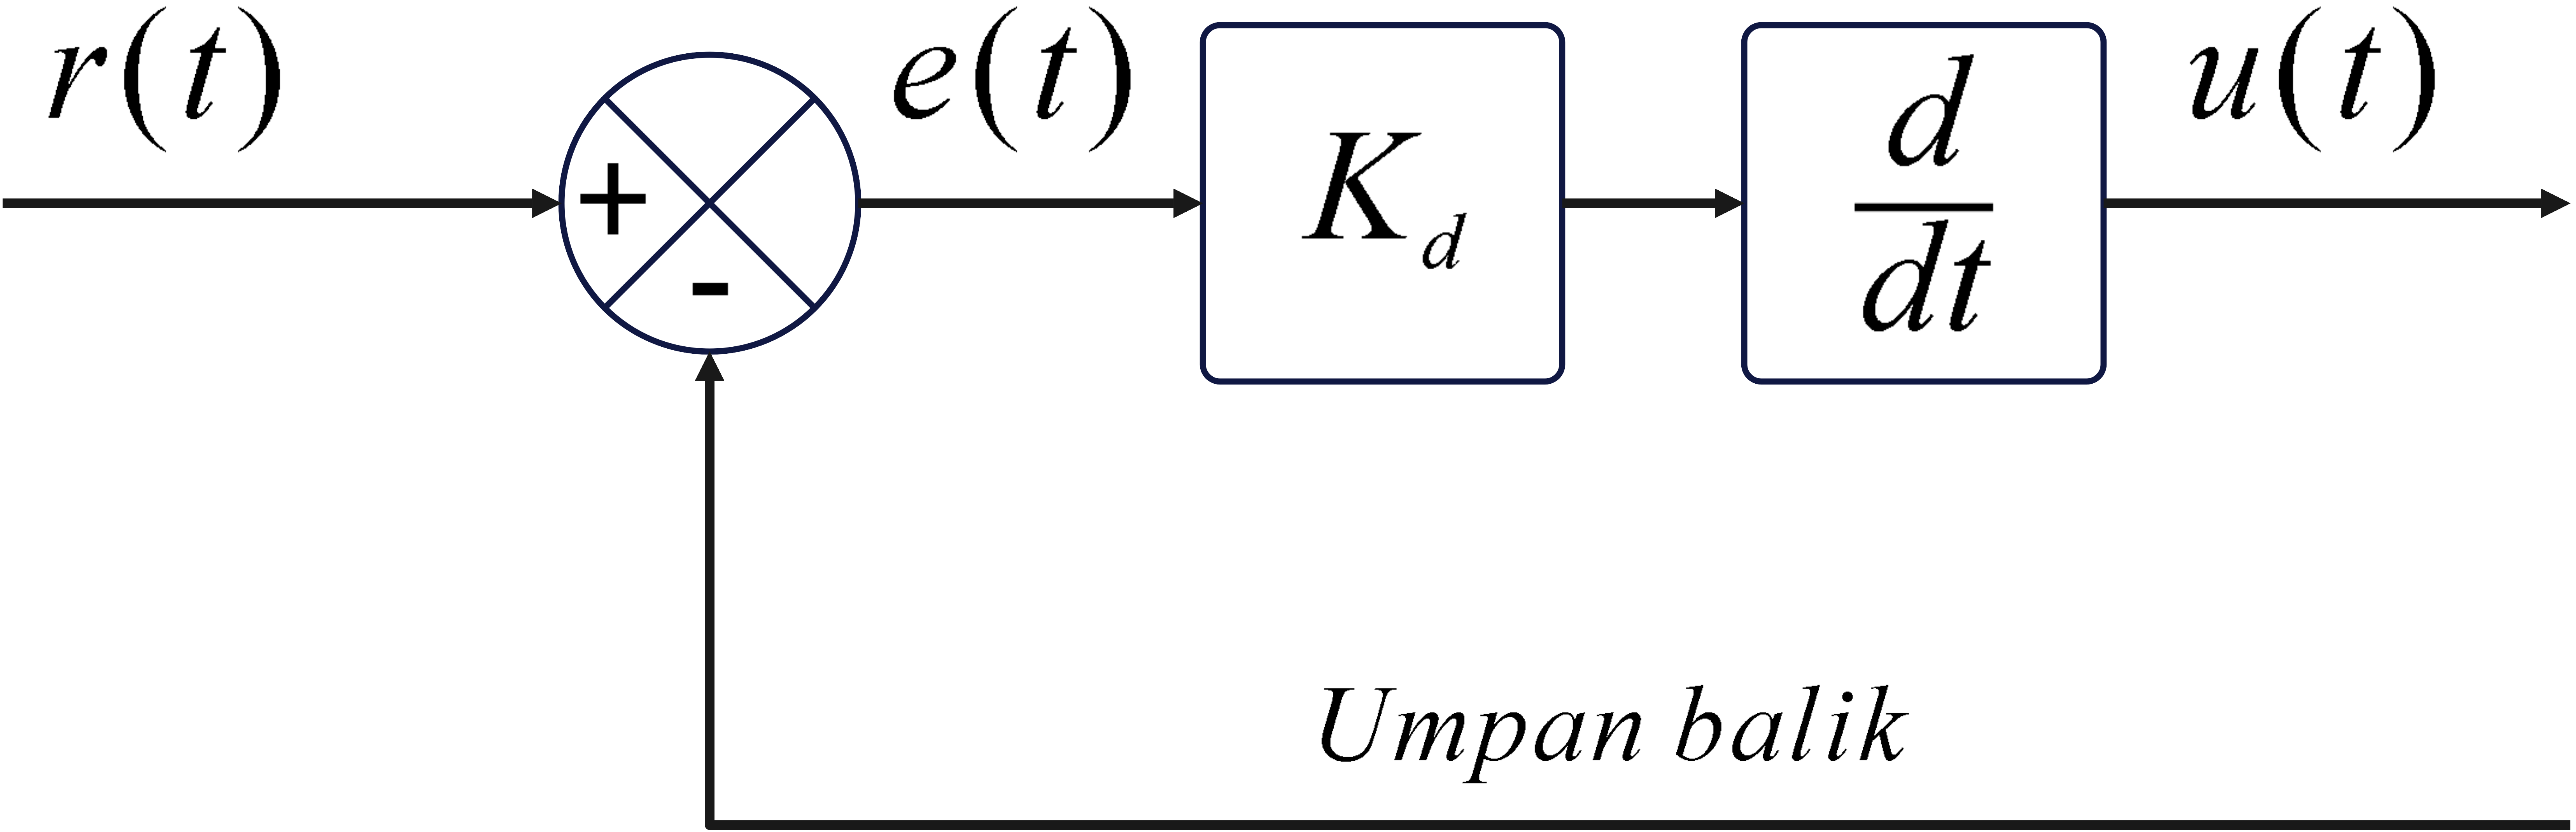
\includegraphics[width=0.8\linewidth]{gambar/diagram.png}
    \caption{Contoh gambar 1}
    \label{gambar1}
\end{figure}

\lipsum[1]

\subsection{Sub Penjelasan Tahapan Penelitian 1}
\lipsum[1]

\section{Penjelasan Tahapan Penelitian 2}
\lipsum[1]

\subsection{Sub Penjelasan Tahapan Penelitian 2}
\lipsum[1]

\begin{table}[H]
	\centering
	\caption{Contoh tabel 3}
	\label{t alpha}
	\begin{tabular}{|c|cccccccc|}
		\hline
		\rowcolor[HTML]{000000} 
		{\color[HTML]{333333} }                                                    & \multicolumn{8}{c|}{\cellcolor[HTML]{000000}{\color[HTML]{FFFFFF} $\dot{e}(k)$}} \\ \hline
		\rowcolor[HTML]{9B9B9B} 
		\cellcolor[HTML]{000000}{\color[HTML]{FFFFFF} }                            & \multicolumn{1}{c|}{\cellcolor[HTML]{9B9B9B}{\color[HTML]{333333} }}   & \multicolumn{1}{c|}{\cellcolor[HTML]{9B9B9B}{\color[HTML]{333333} NB}} & \multicolumn{1}{c|}{\cellcolor[HTML]{9B9B9B}{\color[HTML]{333333} NM}} & \multicolumn{1}{c|}{\cellcolor[HTML]{9B9B9B}{\color[HTML]{333333} NS}} & \multicolumn{1}{c|}{\cellcolor[HTML]{9B9B9B}{\color[HTML]{333333} ZO}} & \multicolumn{1}{c|}{\cellcolor[HTML]{9B9B9B}{\color[HTML]{333333} PS}} & \multicolumn{1}{c|}{\cellcolor[HTML]{9B9B9B}{\color[HTML]{333333} PM}} & {\color[HTML]{333333} PB} \\ \cline{2-9} 
		\rowcolor[HTML]{FFFFFF} 
		\cellcolor[HTML]{000000}{\color[HTML]{FFFFFF} }                            & \multicolumn{1}{c|}{\cellcolor[HTML]{9B9B9B}{\color[HTML]{333333} NB}} & \multicolumn{1}{c|}{\cellcolor[HTML]{FFFFFF}{\color[HTML]{333333} S}}  & \multicolumn{1}{c|}{\cellcolor[HTML]{FFFFFF}{\color[HTML]{333333} S}}  & \multicolumn{1}{c|}{\cellcolor[HTML]{FFFFFF}{\color[HTML]{333333} S}}  & \multicolumn{1}{c|}{\cellcolor[HTML]{FFFFFF}{\color[HTML]{333333} S}}  & \multicolumn{1}{c|}{\cellcolor[HTML]{FFFFFF}{\color[HTML]{333333} S}}  & \multicolumn{1}{c|}{\cellcolor[HTML]{FFFFFF}{\color[HTML]{333333} S}}  & {\color[HTML]{333333} S}  \\ \cline{2-9} 
		\rowcolor[HTML]{FFFFFF} 
		\cellcolor[HTML]{000000}{\color[HTML]{FFFFFF} }                            & \multicolumn{1}{c|}{\cellcolor[HTML]{9B9B9B}{\color[HTML]{333333} NM}} & \multicolumn{1}{c|}{\cellcolor[HTML]{FFFFFF}{\color[HTML]{333333} MS}}  & \multicolumn{1}{c|}{\cellcolor[HTML]{FFFFFF}{\color[HTML]{333333} MS}}  & \multicolumn{1}{c|}{\cellcolor[HTML]{FFFFFF}{\color[HTML]{333333} S}}  & \multicolumn{1}{c|}{\cellcolor[HTML]{FFFFFF}{\color[HTML]{333333} S}}  & \multicolumn{1}{c|}{\cellcolor[HTML]{FFFFFF}{\color[HTML]{333333} S}}  & \multicolumn{1}{c|}{\cellcolor[HTML]{FFFFFF}{\color[HTML]{333333} MS}}  & {\color[HTML]{333333} MS}  \\ \cline{2-9} 
		\rowcolor[HTML]{FFFFFF} 
		\cellcolor[HTML]{000000}{\color[HTML]{FFFFFF} }                            & \multicolumn{1}{c|}{\cellcolor[HTML]{9B9B9B}{\color[HTML]{333333} NS}} & \multicolumn{1}{c|}{\cellcolor[HTML]{FFFFFF}{\color[HTML]{333333} M}}  & \multicolumn{1}{c|}{\cellcolor[HTML]{FFFFFF}{\color[HTML]{333333} MS}}  & \multicolumn{1}{c|}{\cellcolor[HTML]{FFFFFF}{\color[HTML]{333333} MS}}  & \multicolumn{1}{c|}{\cellcolor[HTML]{FFFFFF}{\color[HTML]{333333} S}}  & \multicolumn{1}{c|}{\cellcolor[HTML]{FFFFFF}{\color[HTML]{333333} MS}}  & \multicolumn{1}{c|}{\cellcolor[HTML]{FFFFFF}{\color[HTML]{333333} MS}}  & {\color[HTML]{333333} M}  \\ \cline{2-9} 
		\rowcolor[HTML]{FFFFFF} 
		\cellcolor[HTML]{000000}{\color[HTML]{FFFFFF} }                            & \multicolumn{1}{c|}{\cellcolor[HTML]{9B9B9B}{\color[HTML]{333333} ZO}} & \multicolumn{1}{c|}{\cellcolor[HTML]{FFFFFF}{\color[HTML]{333333} B}}  & \multicolumn{1}{c|}{\cellcolor[HTML]{FFFFFF}{\color[HTML]{333333} M}}  & \multicolumn{1}{c|}{\cellcolor[HTML]{FFFFFF}{\color[HTML]{333333} MS}}  & \multicolumn{1}{c|}{\cellcolor[HTML]{FFFFFF}{\color[HTML]{333333} MS}}  & \multicolumn{1}{c|}{\cellcolor[HTML]{FFFFFF}{\color[HTML]{333333} MS}}  & \multicolumn{1}{c|}{\cellcolor[HTML]{FFFFFF}{\color[HTML]{333333} M}}  & {\color[HTML]{333333} B}  \\ \cline{2-9} 
		\rowcolor[HTML]{FFFFFF} 
		\cellcolor[HTML]{000000}{\color[HTML]{FFFFFF} }                            & \multicolumn{1}{c|}{\cellcolor[HTML]{9B9B9B}{\color[HTML]{333333} PS}} & \multicolumn{1}{c|}{\cellcolor[HTML]{FFFFFF}{\color[HTML]{333333} M}}  & \multicolumn{1}{c|}{\cellcolor[HTML]{FFFFFF}{\color[HTML]{333333} MS}}  & \multicolumn{1}{c|}{\cellcolor[HTML]{FFFFFF}{\color[HTML]{333333} MS}}  & \multicolumn{1}{c|}{\cellcolor[HTML]{FFFFFF}{\color[HTML]{333333} S}}  & \multicolumn{1}{c|}{\cellcolor[HTML]{FFFFFF}{\color[HTML]{333333} MS}}  & \multicolumn{1}{c|}{\cellcolor[HTML]{FFFFFF}{\color[HTML]{333333} MS}}  & {\color[HTML]{333333} M}  \\ \cline{2-9} 
		\rowcolor[HTML]{FFFFFF} 
		\cellcolor[HTML]{000000}{\color[HTML]{FFFFFF} }                            & \multicolumn{1}{c|}{\cellcolor[HTML]{9B9B9B}{\color[HTML]{333333} PM}} & \multicolumn{1}{c|}{\cellcolor[HTML]{FFFFFF}{\color[HTML]{333333} MS}}  & \multicolumn{1}{c|}{\cellcolor[HTML]{FFFFFF}{\color[HTML]{333333} MS}}  & \multicolumn{1}{c|}{\cellcolor[HTML]{FFFFFF}{\color[HTML]{333333} S}}  & \multicolumn{1}{c|}{\cellcolor[HTML]{FFFFFF}{\color[HTML]{333333} S}}  & \multicolumn{1}{c|}{\cellcolor[HTML]{FFFFFF}{\color[HTML]{333333} S}}  & \multicolumn{1}{c|}{\cellcolor[HTML]{FFFFFF}{\color[HTML]{333333} MS}}  & {\color[HTML]{333333} MS}  \\ \cline{2-9} 
		\rowcolor[HTML]{FFFFFF} 
		\multirow{-8}{*}{\cellcolor[HTML]{000000}{\color[HTML]{FFFFFF} $e(k)$}} & \multicolumn{1}{c|}{\cellcolor[HTML]{9B9B9B}{\color[HTML]{333333} PB}} & \multicolumn{1}{c|}{\cellcolor[HTML]{FFFFFF}{\color[HTML]{333333} S}}  & \multicolumn{1}{c|}{\cellcolor[HTML]{FFFFFF}{\color[HTML]{333333} S}}  & \multicolumn{1}{c|}{\cellcolor[HTML]{FFFFFF}{\color[HTML]{333333} S}}  & \multicolumn{1}{c|}{\cellcolor[HTML]{FFFFFF}{\color[HTML]{333333} S}}  & \multicolumn{1}{c|}{\cellcolor[HTML]{FFFFFF}{\color[HTML]{333333} S}}  & \multicolumn{1}{c|}{\cellcolor[HTML]{FFFFFF}{\color[HTML]{333333} S}}  & {\color[HTML]{333333} S}  \\ \hline
	\end{tabular}
\end{table}

\lipsum[1]
\chapter[RENCANA DAN JADWAL KEGIATAN]{\\ RENCANA DAN JADWAL KEGIATAN}

\section{Jadwal Kerja PA}
\lipsum[2][4]

\begin{table}[h!]
    \centering
    \caption{Tabel Rencana Kegiatan (contoh)}
    \begin{tabular}{|c|p{2.5cm}|c|c|c|c|c|c|p{3.5cm}|}
    \hline
    \multirow{2}{*}{\textbf{No}} & \multirow{2}{*}{\textbf{Kegiatan}} & \multicolumn{6}{c|}{\textbf{Bulan}} & \multirow{2}{*}{\textbf{Target capaian}} \\ \cline{3-8} 
    
    & & \textbf{Des} & \textbf{Jan} & \textbf{Feb} & \textbf{Mar} & \textbf{Apr} & \textbf{Mei} & \\ \hline
    
    1 & Studi Literatur & \cellcolor[HTML]{C0C0C0} & \cellcolor[HTML]{C0C0C0} & \cellcolor[HTML]{C0C0C0} & & & & Pengetahuan tentang penelitian sebelumnya dan memahami RL dan MADDPG \\ \hline
    2 & Perancangan awal sistem & & \cellcolor[HTML]{C0C0C0} & \cellcolor[HTML]{C0C0C0} & & & & Merancang garis besar dengan mencari referensi sumber terbuka \\ \hline
    3 & Pengerjaan sistem & & & \cellcolor[HTML]{C0C0C0} & \cellcolor[HTML]{C0C0C0} & & & Pengerjaan simulasi dan sistem MADDPG \\ \hline
    4 & Pengujian sistem & & & & \cellcolor[HTML]{C0C0C0} & \cellcolor[HTML]{C0C0C0} & & Pengujian simulasi dan sistem MADDPG \\ \hline
    5 & Pengambilan data & & & & \cellcolor[HTML]{C0C0C0} & \cellcolor[HTML]{C0C0C0} & & Pengambilan data latih dan data testing \\ \hline
    6 & Pengerjaan sistem & & & & & \cellcolor[HTML]{C0C0C0} & \cellcolor[HTML]{C0C0C0} & Pembuatan laporan \\ \hline
    \end{tabular}
\end{table}



\clearpage
\phantomsection
\addcontentsline{toc}{chapter}{DAFTAR PUSTAKA}
\renewcommand\bibname{DAFTAR PUSTAKA}
\nocite{*}
\bibliography{bibliography/pustaka}
\appendix
\chapter*{LAMPIRAN}
\addcontentsline{toc}{chapter}{LAMPIRAN}
\setcounter{section}{0} % Mengatur ulang penomoran section
\setcounter{page}{1}

\renewcommand{\thesection}{\Alph{section}}
\renewcommand{\thesubsection}{\Alph{section}.\arabic{subsection}\hspace{-0.25cm}}
\renewcommand{\thepage}{L - \arabic{page}}

\begin{center}
    \textit{bila diperlukan}
\end{center}
\end{document}

